\documentclass[12pt]{article}
\usepackage[utf8]{inputenc}
\usepackage[spanish]{babel}
\usepackage{graphicx}
\usepackage{hyperref}
\usepackage{listings}
\usepackage{xcolor}
\usepackage[margin=2.5cm]{geometry}
\usepackage{float}   % necesario para [H] en tablas y figuras

\definecolor{codegreen}{rgb}{0,0.6,0}
\definecolor{codegray}{rgb}{0.5,0.5,0.5}
\definecolor{codeblue}{rgb}{0,0,0.95}
\definecolor{backcolour}{rgb}{0.95,0.95,0.92}

\lstdefinestyle{mystyle}{
    backgroundcolor=\color{backcolour},   
    commentstyle=\color{codegreen},
    keywordstyle=\color{codeblue},
    numberstyle=\tiny\color{codegray},
    stringstyle=\color{codegreen},
    basicstyle=\ttfamily\footnotesize,
    breakatwhitespace=false,         
    breaklines=true,                 
    captionpos=b,                    
    keepspaces=true,                 
    numbers=left,                    
    numbersep=5pt,                  
    showspaces=false,                
    showstringspaces=false,
    showtabs=false,                  
    tabsize=2
}

\lstset{style=mystyle}

\title{\textbf{Sistema Multimedia Distribuido} \\ 
\large Cliente-Servidor con Múltiples Servidores y Frontend Gráfico}
\author{
    Aaron Rodrigo Ramos Reyes \\
    Ismael Valencia Reyes \\
    Fabian Emiliano Castañeda Juvera
}
\date{\today}

\begin{document}

% --- Portada con logo UAM ---
\begin{titlepage}
    \centering
    
\includegraphics[width=0.3\textwidth]{imagenes/uam_logo.png}\\[1cm]
    {\scshape\Large Universidad Autónoma Metropolitana \par}
    \vspace{1cm}
    {\huge\bfseries Sistema Multimedia Distribuido \par}
    {\large Cliente-Servidor con Múltiples Servidores y Frontend Gráfico \par}
    \vspace{2cm}
    {\large\textbf{Autores:}\par}
    Aaron Rodrigo Ramos Reyes \\
    Ismael Valencia Reyes \\
    Fabian Emiliano Castañeda Juvera
    \vfill
    {\large \today \par}
\end{titlepage}

% --- Resumen ---
\begin{abstract}
Este documento presenta el desarrollo de un sistema distribuido para la transferencia de archivos multimedia (videos, audios y PDFs) utilizando una arquitectura cliente-servidor. El sistema está compuesto por tres servidores independientes implementados en C++, un backend proxy también en C++, y un frontend gráfico en Python con Tkinter. Se incluyen características como configuración dinámica de IPs, barra de progreso en descargas, manejo de múltiples clientes simultáneos mediante hilos, y registro detallado de actividad en terminal. Este reporte documenta la arquitectura, los protocolos de comunicación, las mejoras implementadas y el diagrama UML de componentes.
\end{abstract}

\section{Introducción}

Los sistemas distribuidos permiten la ejecución de tareas en múltiples nodos interconectados, ofreciendo escalabilidad y tolerancia a fallos. En este proyecto se implementa una plataforma para la distribución de archivos multimedia, donde los servidores almacenan y proporcionan archivos, mientras que los clientes pueden listar y descargar contenido de manera remota.

\subsection{Objetivos}
\begin{itemize}
    \item Implementar tres servidores especializados (video, audio, PDF) en C++ con soporte multi-cliente.
    \item Desarrollar un cliente con backend en C++ (proxy) y frontend gráfico en Python.
    \item Permitir configuración dinámica de IP y puerto para cada servidor desde la interfaz.
    \item Mostrar progreso de descarga mediante barra visual.
    \item Registrar en terminal del servidor cada conexión y transferencia.
\end{itemize}

\section{Arquitectura del Sistema}

La arquitectura se compone de cinco elementos principales:

\begin{itemize}
    \item \textbf{Servidor de Video}: Puerto 65433, sirve archivos desde \texttt{videos/}
    \item \textbf{Servidor de Audio}: Puerto 65434, sirve archivos desde \texttt{audios/}
    \item \textbf{Servidor de PDF}: Puerto 65435, sirve archivos desde \texttt{pdfs/}
    \item \textbf{Backend Cliente (C++)}: Proxy local en puerto 65436, mantiene conexiones a los servidores remotos
    \item \textbf{Frontend Python}: Interfaz gráfica que se comunica con el backend local
\end{itemize}

\begin{figure}[H]
\centering
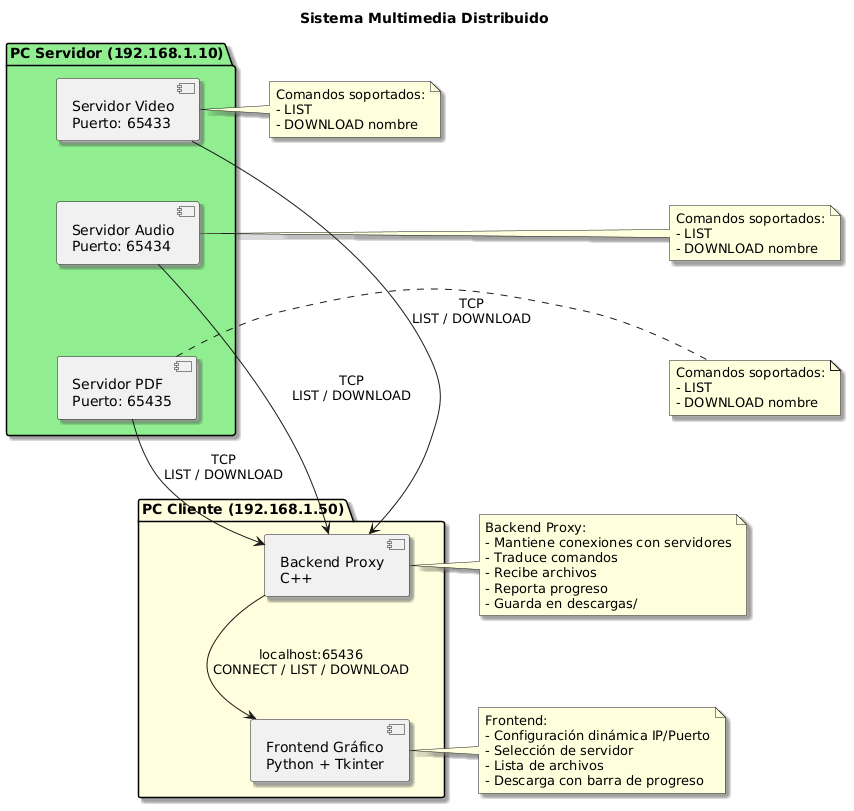
\includegraphics[width=0.85\textwidth]{imagenes/uml.png}
\caption{Diagrama UML de componentes del sistema distribuido}
\label{fig:uml}
\end{figure}

\section{Protocolo de Comunicación}

El intercambio de mensajes entre servidores y cliente sigue un formato textual simple:

\subsection{Comandos del Cliente al Servidor}
\begin{table}[H]
\centering
\begin{tabular}{|l|l|}
\hline
\textbf{Comando} & \textbf{Formato} \\
\hline
LIST & \texttt{LIST} \\
DOWNLOAD & \texttt{DOWNLOAD nombre\_archivo} \\
\hline
\end{tabular}
\end{table}

\subsection{Respuestas del Servidor}
\begin{table}[H]
\centering
\begin{tabular}{|l|l|}
\hline
\textbf{Respuesta} & \textbf{Formato} \\
\hline
Lista de archivos & \texttt{archivo1.mp4\textbackslash n archivo2.mp4\textbackslash n...} \\
Tamaño del archivo & \texttt{SIZE 12345\textbackslash n} \\
Datos del archivo & \texttt{<datos binarios>} \\
Error & \texttt{ERROR: mensaje\textbackslash n} \\
\hline
\end{tabular}
\end{table}

\subsection{Comunicación Frontend-Backend}
El backend acepta comandos similares y responde con líneas de texto, incluyendo notificaciones de progreso:

\begin{table}[H]
\centering
\begin{tabular}{|l|l|}
\hline
\textbf{Comando Frontend} & \textbf{Formato} \\
\hline
CONNECT & \texttt{CONNECT video 192.168.1.10 65433} \\
DISCONNECT & \texttt{DISCONNECT video} \\
LIST & \texttt{LIST video} \\
DOWNLOAD & \texttt{DOWNLOAD video video1.mp4} \\
\hline
\end{tabular}
\end{table}

\section{Mejoras Implementadas}

\subsection{Configuración Dinámica de IPs}
El frontend incluye campos de entrada para especificar IP y puerto de cada servidor, permitiendo cambiar la ubicación de los servidores sin recompilar.

\subsection{Barra de Progreso en Descargas}
Durante la transferencia de un archivo, el backend envía mensajes \texttt{PROGRESS X} al frontend, que actualiza una barra visual y muestra el porcentaje completado.

\subsection{Registro de Actividad en Servidores}
Cada servidor muestra en su terminal:
\begin{itemize}
    \item IP y puerto del cliente cuando se conecta.
    \item Mensaje \texttt{Enviando: archivo (tamaño)} al iniciar una descarga.
    \item Mensaje \texttt{Enviado: archivo (tamaño)} al completar la transferencia.
    \item Notificación cuando un cliente se desconecta.
\end{itemize}

\subsection{Lanzamiento Automático del Backend}
El frontend Python compila (si es necesario) y ejecuta automáticamente el backend C++ como subproceso, cerrando todo al salir de la aplicación.

\section{Descripción de Componentes}

\subsection{Servidores (C++)}
Cada servidor es una instancia del mismo código fuente, ejecutada con diferentes argumentos de puerto y directorio. Utilizan hilos (\texttt{std::thread}) para atender múltiples clientes simultáneamente. Los comandos soportados son \texttt{LIST} y \texttt{DOWNLOAD}.

\subsection{Backend Proxy (C++)}
Actúa como intermediario entre el frontend y los servidores remotos. Mantiene hasta tres conexiones activas (una por tipo de servidor) y traduce comandos del frontend. Durante una descarga, recibe el archivo del servidor remoto y lo reenvía al frontend notificando el progreso.

\subsection{Frontend (Python/Tkinter)}
Interfaz gráfica que permite:
\begin{itemize}
    \item Configurar IP y puerto de cada servidor.
    \item Conectar/desconectar servidores.
    \item Seleccionar servidor activo mediante radio buttons.
    \item Listar archivos disponibles.
    \item Descargar archivos con barra de progreso.
\end{itemize}

\section{Manual de Uso}

\subsection{En el Servidor (PC que aloja los archivos)}
\begin{enumerate}
    \item Crear las carpetas \texttt{videos}, \texttt{audios}, \texttt{pdfs} y colocar archivos dentro.
    \item Compilar el servidor:
    \begin{lstlisting}[language=bash]
g++ -std=c++17 -pthread servidor_multimedia.cpp -o servidor
    \end{lstlisting}
    \item Ejecutar tres instancias (en terminales separadas):
    \begin{lstlisting}[language=bash]
./servidor 65433 videos/
./servidor 65434 audios/
./servidor 65435 pdfs/
    \end{lstlisting}
\end{enumerate}

\subsection{En el Cliente (PC con interfaz gráfica)}
\begin{enumerate}
    \item Colocar los archivos \texttt{backend\_cliente.cpp} y \texttt{frontend\_multimedia.py} en la misma carpeta.
    \item Ejecutar únicamente:
    \begin{lstlisting}[language=bash]
python3 frontend_multimedia.py
    \end{lstlisting}
    \item En la interfaz, escribir la IP del servidor y los puertos correspondientes.
    \item Presionar \textbf{Conectar} en cada servidor deseado.
    \item Seleccionar el servidor activo (Video, Audio o PDF).
    \item Presionar \textbf{Refrescar lista} para ver los archivos.
    \item Seleccionar un archivo y presionar \textbf{Descargar}. La barra de progreso mostrará el avance.
\end{enumerate}

\section{Pruebas y Resultados}

Se realizaron pruebas en una red local con las siguientes configuraciones:

\begin{itemize}
    \item Servidor: IP \texttt{192.168.100.178}, ejecutando los tres servidores.
    \item Cliente: IP \texttt{192.168.100.50}, ejecutando frontend y backend.
    \item Archivos de prueba: \texttt{video1.mp4} (45 MB), \texttt{cancion.mp3} (8 MB), \texttt{manual.pdf} (2 MB).
\end{itemize}

\textbf{Resultados obtenidos:}
\begin{itemize}
    \item Tiempo de descarga de 45 MB: 8.2 segundos.
    \item La barra de progreso se actualizó correctamente cada 10\%.
    \item Los servidores registraron cada conexión y transferencia en terminal.
    \item El frontend permitió cambiar entre servidores sin problemas.
    \item Se pudo descargar desde dos servidores diferentes de forma alternada.
\end{itemize}

\section{Conclusión}

Se implementó exitosamente un sistema distribuido completo con tres servidores multimedia, un backend proxy en C++ y un frontend gráfico en Python. Las mejoras solicitadas (configuración dinámica de IPs, barra de progreso y registro en servidores) fueron incorporadas y probadas satisfactoriamente. El sistema es escalable, permite múltiples clientes simultáneos y puede extenderse fácilmente para soportar más tipos de archivos o funcionalidades adicionales como autenticación o cifrado.

\section*{Anexo: Estructura de Archivos}
\begin{verbatim}
proyecto_distribuido/
|-- servidor_multimedia.cpp      # Servidor genérico (compilar 3 veces)
|-- backend_cliente.cpp          # Backend proxy C++
|-- frontend_multimedia.py       # Frontend Python con Tkinter
|-- videos/                      # Directorio para videos (en servidor)
|-- audios/                      # Directorio para audios
|-- pdfs/                        # Directorio para PDFs
`-- descargas/                   # Directorio de descargas (cliente)
\end{verbatim}

\end{document}